\section{Validity of the dimension-6 interpretation}
\label{sec:truncation}

\label{sec:trunc_convergence}
Truncating the SMEFT expansion at dimension six has consequences for an \HH analysis and
for the tools of this report, and this section works out three of them. The first is the
range of each Wilson coefficient over which the chosen truncation is one an analysis
would want. The second is the order at which a product such as
$\sigma\times\mathrm{BR}$ is truncated. The third is the region of
$c_{\PH\mathrm{kin}}$ in which the prediction is physical at all. 

Whether a dimension-6 description is adequate, and where it stops being adequate, has a
literature of its own. The standard prescription keeps the coefficients in the region
where the interference dominates the dimension-6 square, and the threshold is a
convention: requiring the square to be below the interference, or below some fraction of
it, has no first-principles
answer~\cite{Contino:2016jqw,Brivio:2017vri}.
That choice is not settled here. Appendix~\ref{sec:appendix_trunc_validity} tabulates
the coupling value at which the square equals the interference, for each leading
operator and in each \mHH bin, so that an analysis can apply whichever convention it
adopts.

Because the coefficients are extracted bin by bin, the relative weight of the linear and
quadratic brackets is a function of the kinematics and differs from operator to operator.
Table~\ref{tab:trunc_validity} of Appendix~\ref{sec:appendix_trunc_validity} gives, for
each leading operator, the coupling value at which the two contribute equally, $|A^j_{\text{quad}}c^2|=|A^j_{\text{lin}}c|$, that is
$|c|\simeq|A^j_{\text{lin}}/A^j_{\text{quad}}|$, inclusively and in three \mHH bins. The
quantity exists only for the four leading operators, the ones with a genuine square;
$A^j_{\text{quad}}$ is the corresponding diagonal entry $A^j_5$, $A^j_9$, $A^j_{12}$ or
$A^j_{14}$.

The pattern is not common to the four. For $c_\PH$ the bound \emph{loosens} with \mHH, from
$9$ near threshold to $28$ above $1.4$~TeV: it rescales the trilinear coupling and so enters
only the $s$-channel triangle, whose amplitude falls relative to the box as the invariant
mass grows, so both its brackets die out in the tail and the truncation error it induces is
a threshold effect. For the other three the bound tightens with \mHH, by a factor $8$ for
$c_{\PH\mathrm{kin}}$, $11$ for $c_{\PQt\PH}$ and $13$ for $c_{\PH G}$ between the bin at
$400$~GeV and the one at $1.4$~TeV. $c_{\PQt\PH}$ scales the box contribution, which
dominates above threshold; $c_{\PH G}$ generates point-like $\PH\Pg\Pg$ and $\HH\Pg\Pg$
interactions that do not carry the loop suppression of the SM amplitude, so the
ratio of its square to its interference grows with the momentum transfer, and it has by far
the tightest bound of the four.

For all four leading operators the generated ranges of Table~\ref{tab:SMEFTcouplings} extend
beyond the inclusive bound, and in the tail the margin is larger still: $c_{\PH G}$ is
generated to $-0.1$ against an inclusive bound of $0.026$ and a bound of $0.006$ above
$1.4$~TeV. The ranges were chosen to cover the region experiments probe, not the region in
which the expansion converges, and the two are not the same. The practical consequence is
that an inclusive statement about the truncation is weaker than a differential one: a
coefficient value at which the inclusive cross section is insensitive to the truncation can
still change the high-mass tail by a large factor, and it is the tail that most \HH analyses
exploit.

That value is not a confidence interval and not a bound on new physics. It is the
coupling value at which the dimension-6 squared contribution becomes as large as the
dimension-6 interference in the bin considered; at that value the formally higher-order
terms the parameterization does not contain, in particular the dimension-8 interference
with the SM, which is of the same $1/\Lambda^4$ order as the dimension-6 square,
can no longer be argued to be negligible. Being a per-bin quantity, the bound from a
high-mass bin is tighter than the inclusive one, and the tighter number is the relevant one
whenever a shape fit uses the tail. It concerns the convergence of the $1/\Lambda^2$
expansion at the scale of the process and says nothing about the renormalization-group
running of the coefficients, which Eq.~\eqref{eq:smeftpara_reorg} assumes to be absent
(Sec.~\ref{sec:parameterization})~\cite{Heinrich:2024rtg}.

The subleading operators behave differently by construction. They appear linearly in
$A^j_{15}$--$A^j_{19}$ and quadratically only through the mixed block
$A^j_{20}$--$A^j_{39}$, which multiplies them by a leading coefficient. Along a
one-dimensional ray in which a single subleading coefficient is varied and the leading ones
are at zero, the parameterization is exactly linear and the truncation ratio is identically
unity; the quadratic effect of $c_{\PQt G}$, $c_{Q\PQt}^{(1)}$, $c_{Q\PQt}^{(8)}$,
$c_{QQ\PQt\PQt}$ and $c_{QQ}^{(8)}$ is visible only where a leading coefficient is also
switched on. No validity bound of the above kind exists for them.

\textcolor{red}{MATHEUS, OSCAR do you agree? Or we remove that.}

Two limitations remain. The purely subleading squares are absent from the generation and
cannot be recovered from these coefficients; quantifying them needs a dedicated sample.
And the four benchmarks of Fig.~\ref{fig:linearquad} vary only $c_\PH$,
$c_{\PH\mathrm{kin}}$ and $c_{\PQt\PH}$, so the operator with the strongest energy growth,
$c_{\PH G}$, is at zero in every one of them; the hierarchy of
Appendix~\ref{sec:appendix_trunc_validity} is therefore not tested against simulation.

The coefficients are extracted independently at each energy
(Sec.~\ref{sec:extraction}), so the same ratios can be evaluated wherever a
determination exists. The consequences for an analysis that must supply
linear-truncation templates after a realistic selection are taken up in
Sec.~\ref{sec:validation_realistic}.

\label{sec:trunc_product}
The second statement concerns a quantity that is a product. What an analysis predicts is
not a cross section but $\sigma\times\mathrm{BR}$, and the order of the expansion has to
be applied to that product rather than to its factors. Expanding the production and each
partial width to first order in $\kappa_\lambda-1$ and then multiplying is not the same
operation: it retains a $\sigma_{\text{lin}}\times\mathrm{BR}_{\text{lin}}$ cross term
that is second order in the Wilson coefficients, while $1/\Gamma_{\text{tot}}$ has to be
expanded as a series before it can be truncated at all.

The size of the difference is set by the \ttH channel, whose cross section has
the largest $C_1$, $3.51\%$, from the Higgs boson radiated off top quarks near threshold:
a unit change of $c_\PH$ at $\Lambda=1$~TeV moves it by $1.5\%$, against $0.15\%$ for
gluon fusion. The $Z_\PH$ factor is quadratic in $\kappa_\lambda$, so the cross sections
are not monotonic; \ttH reaches $1.14$ times its SM value at $c_\PH\simeq-19$. Truncating the factors rather than the
product leaves $\sigma\times\mathrm{BR}$ within $1\%$ of the
full form for $|c_\PH|\lesssim5$, $3$--$4\%$ at $c_\PH=10$, and up to a factor of two at
the edges of the range, the growth coming mainly through $Z_\PH$.

The recommendation is to truncate the product once, at the order the analysis claims,
and not the factors separately; this is what the reference implementation of
Ref.~\cite{multihmodels} does, expanding $1/\Gamma_{\text{tot}}$ as a series and then the
full product, with the truncation order applied to the final $\sigma\times\mathrm{BR}$.
This is not a matter of convention. Truncating the factors separately retains a term of
second order in the Wilson coefficients while claiming a first-order result, so it is
inconsistent whatever the numerical difference happens to be. The numbers above say how much it costs, which is what is
needed to judge a result produced the other way: below $|c_\PH|\simeq5$ the two agree within $1\%$ and such a result can be used
as it stands, while at the edges of the range the difference exceeds any uncertainty the
analysis would otherwise quote.

This choice does not enter the construction of the templates. The bases
of Sec.~\ref{sec:basisopt} are optimized on cross sections and are agnostic to the Higgs
decay: no branching ratio enters the parameterization, the morphing or the basis
selection. The truncation of a product is therefore a property of the final application,
fixed by the analysis when it forms $\sigma\times\mathrm{BR}$, and not a property of the
templates it is given.

\textcolor{red}{\textbf{Oscar, Jon:} do you agree with stating this as a
recommendation --- that the expansion order be applied once to the final
$\sigma\times\mathrm{BR}$ rather than to its factors?}

\subsection{Single-Higgs interplay and the physical region of
\texorpdfstring{$c_{\PH\mathrm{kin}}$}{cHkin}}
\label{sec:trunc_singleh}
\label{sec:singleh}
\label{sec:singleh_naive}

The nine Wilson coefficients of Eq.~\eqref{eq:smeftpoint} also enter single-Higgs
production and decay, so a global fit constrains them with single-\PH and \HH data
together. The operator $(\phi^\dagger\phi)^3$ modifies no single-Higgs vertex at tree
level and enters only through the trilinear vertex in electroweak loop
corrections~\cite{Degrassi:2016wml,Maltoni:2017ims}; the resulting dependence is
parameterized by the process- and kinematics-dependent coefficients $C_1$ provided by
the LHC Higgs Working Group, and carried through to the simplified template cross
sections (STXS) used for single-Higgs measurements, where the $C_1^i$ are derived per
STXS bin
with a common ATLAS and CMS
convention~\cite{ATLAS:2024lyh,Berger:2019wnu,Brivio:2022pyi,Belvedere:2024nzh}. The
translation between $\kappa_\lambda$ and the Warsaw-basis coefficient is standard in
global SMEFT analyses. None of that is specific to this report, and an analysis
combining single-\PH and \HH should take it from those references.

What does not follow from them is the truncation at which the two sides meet. The \HH
parameterization of this report is quadratic in $c_\PH$, the single-Higgs scaling is a
one-loop effect entering at $\mathcal{O}(\Lambda^{-2})$ and is used linearly, and
$\sigma\times\mathrm{BR}$ is not the product of two truncated factors
(Sec.~\ref{sec:trunc_product}). A combination has to state which truncation it applies
on each side and over what range that choice is valid. The ranges below and in
Sec.~\ref{sec:trunc_convergence} are derived with the conventions used for the \HH
templates, so that the two sides refer to the same $c_\PH$.

\textcolor{red}{The implementation behind the single-Higgs numbers quoted here is in
Appendix~\ref{sec:appendix_singleh}, which is for the authors: it is our own code, kept
to check that implementation against what the literature already provides, not a result
of this report.}

The remaining statement concerns positivity rather than the expansion. The
coefficient $c_{\PH\mathrm{kin}}$ multiplies the Higgs kinetic term, and removing it by a
field redefinition rescales \emph{every} single-Higgs coupling by the same factor, the
top--Higgs coupling included.

An \HH analysis intending a SMEFT interpretation can constrain that coefficient with
data it already has. Several of the main \HH channels contain \ttH-enriched regions,
because \ttH is a leading background there. If those regions are given the
same coefficient dependence as the signal rather than a freely floating normalization,
they constrain $c_{\PH\mathrm{kin}}$ through the common rescaling of the top--Higgs
coupling, using data the analysis has already collected. That constraint is what keeps a
fit inside the physical region below: an \HH-only likelihood that leaves
$c_{\PH\mathrm{kin}}$ to the \HH rate alone can wander past the point where the
partial widths it implicitly assumes have gone negative, and nothing in the \HH
prediction signals it.

\textcolor{red}{\textbf{Oscar, Jon:} is this recommendation one we want to make ---
that \HH analyses aiming at a SMEFT interpretation parameterize their \ttH-enriched
regions in the same coefficients rather than floating them? We have not quantified how
much it tightens $c_{\PH\mathrm{kin}}$ relative to the \HH rate alone.}

The ingredients of the physical region are the naive translation between the self-coupling modifier and the Warsaw
basis~\cite{Alasfar:2023xpc},
%
\begin{equation}
\kappa_\lambda
= 1 - 2\,\frac{v^2}{\Lambda^2}\frac{v^2}{m_\PH^2}\,c_\PH
+ 3\,\frac{v^2}{\Lambda^2}\,c_{\PH\mathrm{kin}} ,
\label{eq:naivetranslation}
\end{equation}
%
which with $v=246.22$~GeV, $m_\PH=125$~GeV and $\Lambda=1$~TeV gives a coefficient of
$c_\PH$ of $-0.470$, so that $c_\PH\in[-50,50]$ of Table~\ref{tab:SMEFTcouplings} maps
onto $\kappa_\lambda\in[-22.5,24.5]$; and the scaling of each partial width under that
field redefinition,
%
\begin{equation}
\frac{\Gamma_i}{\Gamma_i^{\mathrm{SM}}}=\left(1+x\right)^2
\;\xrightarrow[\text{linear truncation}]{}\;
1+2x ,
\qquad
x\equiv c_{\PH\mathrm{kin}}\,\frac{v^2}{\Lambda^2} .
\label{eq:chkinwidth}
\end{equation}

Although the branching ratios barely move with $c_{\PH\mathrm{kin}}$, the partial
widths of Eq.~\eqref{eq:chkinwidth} do (Fig.~\ref{fig:sh_physical}, left). The
quadratic form is never negative; the linear one crosses zero at
\begin{equation}
c_{\PH\mathrm{kin}}^{\,0}=-\frac{\Lambda^2}{2v^2}
\;\simeq\;-8.25 \quad (\Lambda=1~\text{TeV}),
\label{eq:chkinzero}
\end{equation}
$0.25$ below the lower edge of the range $[-8,8]$ of
Table~\ref{tab:SMEFTcouplings}, where the linear widths are $3.0\%$ of their SM
values and the quadratic ones $26.5\%$. An analysis with linearly truncated rates,
\HH included since its final states carry two Higgs branching ratios, keeps the
widths and branching ratios positive only for
\begin{equation}
c_{\PH\mathrm{kin}}\;>\;-\frac{\Lambda^2}{2v^2}
\;\simeq\;-8.25\left(\frac{\Lambda}{1~\mathrm{TeV}}\right)^{2} ,
\label{eq:chkinbound}
\end{equation}
shown against $\Lambda$ in Fig.~\ref{fig:sh_physical} (right): the range $[-8,8]$ is
physical for $\Lambda\gtrsim0.99$~TeV. With the quadratic form only
$|c_{\PH\mathrm{kin}}|<\Lambda^2/v^2$ remains, where the Higgs couplings vanish.
The \HH cross section carries higher powers of the same factor: with
$c_\PQt\propto(1+x)$ and $c_{hhh}\propto(1+x)^3$, the box-squared, interference and
triangle-squared terms scale as $(1+x)^4$, $(1+x)^6$ and $(1+x)^8$, whose linear
truncations turn negative at $c_{\PH\mathrm{kin}}=-4.12$, $-2.75$ and $-2.06$ at
$\Lambda=1$~TeV; the strictest, $c_{\PH\mathrm{kin}}>-\Lambda^2/(8v^2)$, is the
dashed curve of Fig.~\ref{fig:sh_physical} (right). The parameterization of this
report keeps the quadratic terms of the leading operators, so its templates are not
affected.

The single-Higgs model of Ref.~\cite{multihmodels} holds two couplings where the STXS
parameterization leaves its range of use. The partial and total widths are linear in
$c_{\PH\Box}$, the partial widths turning negative at $|c_{\PH\Box}|\simeq8.2$, and
$1/\Gamma$ is expanded as $1-x+x^2$, $x=\Gamma/\Gamma_{\mathrm{SM}}-1$, which differs from
the exact $1/\Gamma$ by $3.7\%$ at $|c_{\PH\Box}|=3$ and by $70\%$ at 8; $|c_{\PH\Box}|$
and $|c_{\PH\mathrm{kin}}|$ are held at 3 in the widths, of single Higgs and of the \HH
decays. The quadratic gluon-fusion scaling in $c_{\PH G}$ is negative between its two roots,
the upper one from $-0.033$ to $-0.014$ across the STXS bins; $c_{\PH G}$ is held at
$-0.0136$ and above in the single-Higgs production.

There are therefore two bounds on $c_{\PH\mathrm{kin}}$, and the generated range sits
between them. Positivity of the linearly truncated widths requires
$c_{\PH\mathrm{kin}} > -8.25$ at $\Lambda = 1$~TeV, Eq.~\eqref{eq:chkinbound}, which
the range $[-8,8]$ of Table~\ref{tab:SMEFTcouplings} respects; the expansion of
$1/\Gamma$ stops being usable much earlier, which is why the widths are evaluated at
$|c_{\PH\mathrm{kin}}| \le 3$. A fit that floats $c_{\PH\mathrm{kin}}$ over the full
range is thus clamped in practice over most of it: beyond $|c_{\PH\mathrm{kin}}| = 3$
the single-Higgs and \HH branching ratios no longer move, and the sensitivity comes
from the \HH production, which is never clamped, and from the single-Higgs production,
which is not clamped in this coupling. The same applies to $c_{\PH G}$ below $-0.0136$,
where the gluon-fusion single-Higgs rate is constant while the \HH morphing continues
to vary.

A limit or a contour that ends in those regions is a statement made under the clamp and
should be reported as one. The clamps are not a theory uncertainty: they replace a
prediction that has left its range of validity by a constant, and they do not estimate
the terms that are missing.

\begin{figure}[htp]
\centering
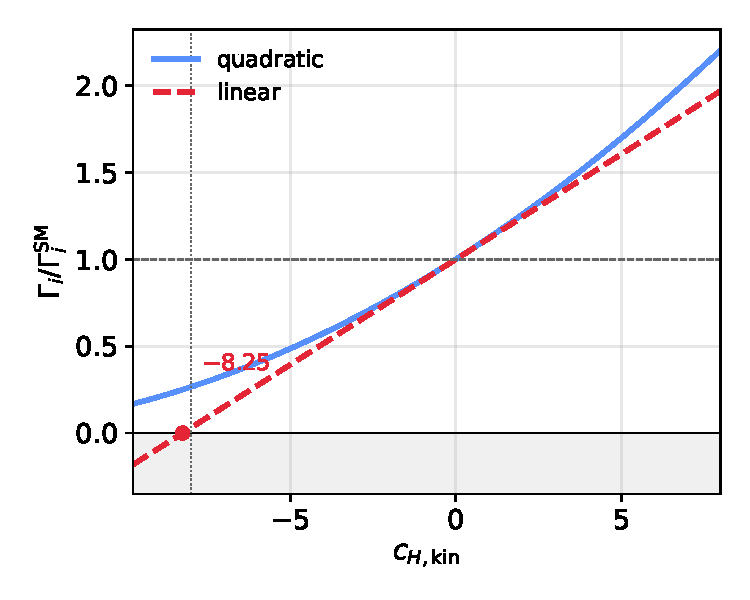
\includegraphics[width=0.49\textwidth]{single_higgs_ch/figures/width_vs_cHkin.pdf}
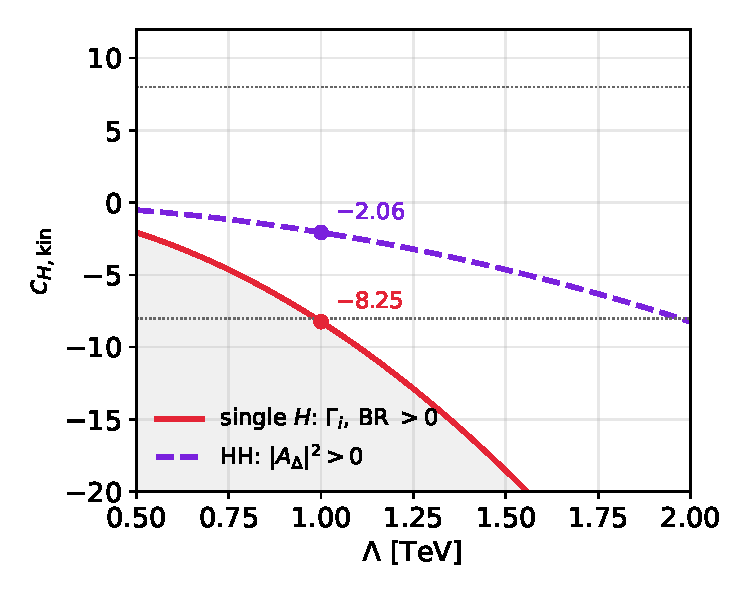
\includegraphics[width=0.49\textwidth]{single_higgs_ch/figures/physical_region_cHkin.pdf}
\caption{Left: single-Higgs partial widths as a function of $c_{\PH\mathrm{kin}}$
at $\Lambda=1$~TeV, Eq.~\eqref{eq:chkinwidth}, in the quadratic (solid) and linear
(dashed) truncations. The grey band marks negative widths, the marker the zero of the
linear form, Eq.~\eqref{eq:chkinzero}, and the dotted line the lower edge of the range
of Table~\ref{tab:SMEFTcouplings}. Right: the lower bound on $c_{\PH\mathrm{kin}}$
for positive linearly truncated rates as a function of $\Lambda$: the single-Higgs
partial widths and branching ratios, Eq.~\eqref{eq:chkinbound} (solid; grey below),
and the \HH triangle-squared term (dashed). The dotted lines mark the range of
Table~\ref{tab:SMEFTcouplings}, the markers the two bounds at $\Lambda=1$~TeV.}
\label{fig:sh_physical}
\end{figure}
